% This template was initially provided by Dulip Withanage.
% Modifications for the database systems research group
% were made by Conny Junghans,  Jannik Strötgen and Michael Gertz

\documentclass[
     12pt,         % font size
     a4paper,      % paper format
     BCOR10mm,     % binding correction
     DIV14,        % stripe size for margin calculation
     ]{article}

%%%%%%%%%%%%%%%%%%%%%%%%%%%%%%%%%%%%%%%%%%%%%%%%%%%%%%%%%%%%

% PACKAGES:

% Use German :
\usepackage[english]{babel}
% Input and font encoding
\usepackage[latin1]{inputenc}
\usepackage[T1]{fontenc}
% Index-generation
\usepackage{makeidx}
% Einbinden von URLs:
\usepackage{url}
% Special \LaTex symbols (e.g. \BibTeX):
%\usepackage{doc}
% Include Graphic-files:
\usepackage{graphicx}
% Include doc++ generated tex-files:
%\usepackage{docxx}

% Fuer anderthalbzeiligen Textsatz
\usepackage{setspace}

\usepackage[title]{appendix}

% hyperrefs in the documents
\PassOptionsToPackage{hyphens}{url}\usepackage[bookmarks=true,colorlinks,pdfpagelabels,pdfstartview = FitH,bookmarksopen = true,bookmarksnumbered = true,linkcolor = black,plainpages = false,hypertexnames = false,citecolor = black,urlcolor=black]{hyperref}
%\usepackage{hyperref}

%%%%%%%%%%%%%%%%%%%%%%%%%%%%%%%%%%%%%%%%%%%%%%%%%%%%%%%%%%%%

% OTHER SETTINGS:

% Choose language
\newcommand{\setlang}[1]{\selectlanguage{#1}\nonfrenchspacing}


\begin{document}

% TITLE:
\pagenumbering{roman} 
\begin{titlepage}


\vspace*{1cm}
\begin{center}
\vspace*{3cm}
\textbf{ 
\Large Heidelberg University\\
\smallskip
\Large Institute of Computer Science\\
\smallskip
\Large Database Systems Research Group\\
\smallskip
}

\vspace{3cm}

\textbf{\large Project Proposal for the lecture Text Analytics}

\vspace{0.5\baselineskip}
{\huge
\textbf{Clustering of scientific papers for easy information retrieval}
}
\end{center}

\vfill 

{\large
\begin{tabular}[l]{ll}
Team Member: & Daniela Fichiu, 3552717, BSc Applied Computer Science,\\
  & BSc Mathematics\\
  & daniela.fichiu@stud.uni-heidelberg.de\\
Team Member: & Christian Homeyer, 3606476, PhD Computer Science \\
  & ox182@uni-heidelberg.de\\
Team Member: & Jessica Kaechele, 3588787, MSc Applied Computer Science\\
  & Uo251@stud.uni-heidelberg.de\\
Team Member: & Jonas Reinwald, 3600238, MSc Applied Computer Science\\
  & am248@stud.uni-Heidelberg.de\\
  
\end{tabular}
}

{
  \textbf{GitHub Repository: \url{https://github.com/DonatJR/ita_ws20}}
}

\end{titlepage}

\pagenumbering{arabic} 
% TODO Add source link to Data repo, this is done in the text and not on frontpage?

\section{Motivation}

Before typing an exact query like "how do I open the terminal on mac?" into a search engine, one already has an exact idea of what he wants to find: a set of steps that will lead to terminal being displayed on the screen. 

When starting a new project or trying to improve existing bodies of work it is often vitally important to do extensive research. This both helps to familiarize oneself with the topic that is to be worked on and provides the necessary new information that is needed to solve the problem at hand.

A student who wants to know more about text analytics might search for "text analytics" on Google Scholar. The query yields back 1.650.000 results, the top three being "Text Analytics with Python", "Text analytics in social media" and "Semantic interaction for visual text analytics". A subsequent query like "text analytics topics" yields back results with the following titles: "Analyzing educational comments for topics and sentiments: A text analytics approach" or "A text analytics approach for online retailing service improvement: Evidence from Twitter". No query has so far returned the expected results.

We know how time-consuming it is to spend hours on search engines or websites like Research Gate or Google Scholar looking for research papers, hoping for the best, but never quite finding what we were looking for.

Our project emerged from the need of finding an easy way of exhaustively searching for scholarly literature, while bringing to light the relations between the subfields of the research field of interest and/or of other fields, thus providing a deeper understanding of the material to be searched for and easing up the process of finding information. We believe that our project will especially benefit people who are just getting started or have little experience with reading or searching for academic papers. 

We want to propose a solution to this by taking scientific texts and clustering them into relevant subgroups, which can then be more easily presented to and explored by people looking for specific topics and terms.

While we intend to first focus on a rather narrow subset of papers from a topic like Deep Learning or something similar, more or less specific subgroups for clustering therein can be explored to find a good balance. The proposed pipeline should later be usable on a broader range of fields.

Furthermore, we think a solution to the stated problem could later be used on a grander scale by building good group visualization tools and providing existing websites with this technology.

In addition, a meta search site incorporating data from these other sources with a common, easily digestible search and presentation interface could be developed.

\section{Research Topic Summary}
There exist various approaches to simplify getting an overview of a research field without extensive research and reading countless papers. Browsing through digital libraries and search engines can yield papers matching search strings, but to get an overview of an entire research area this is not good enough.

In \cite{Rapid_understanding_of_scientific_paper_collections} a tool is presented that uses the citation network to divide papers into clusters and identify trends, gaps and outliers.
Another way to gain insights is to find key statements of a paper. As finding these statements is computationally expensive, the authors use `Multi-Document Summarization' which is only applied to abstracts and citation contexts. The dataset used is ACL Anthology Network (AAN) \cite{aan} and contains the network of citations, as well as the full text of each article, its metadata, summary, references and citation sentences.

These techniques make it possible to gain insight into an entire research field more quickly, but for this project we will concentrate only on the clustering.
Attempts to cluster papers have been made for many years. In 1973, for example, it had already been tried to cluster journals by comparing reference patterns and looking at mutual references \cite{Clustering_of_scientific_journals}.

In \cite{Document_clustering_of_scientific_texts_using_citation_contexts} the context of the citations is used in addition to the citations itself to cluster.
Citations are identified and text around it is extracted to then use link-based clustering approaches, term-based clustering approaches and hierarchical document clustering, as well as a combination of all three, on this data.
For comparison, this technique is also applied to the entire document and contrasted against the approach of using only citation context.

In \cite{Clustering_scientific_documents_with_topic_modeling} abstracts and titles of documents from Web of Science \cite{web_of_science} are used.
They perform two types of pre-processing, the first treats each word as a token, and stopwords are deleted. The second method uses term-clumping to find noun phrases with significant commonality.
Then, several topic modeling algorithms are used: The Latent Dirichlet allocation (LDA), Correlated Topic Models (CTM), Hierarchical Latent Dirichlet Allocation (Hierarchical LDA) and Hierarchical Dirichlet Process (HDP).

Abstracts are also used in \cite{An_Approach_to_Clustering_Abstracts} to perform clustering. They use tokenization, remove stopwords and then apply a stemming algorithm.
Keywords are then grouped and weighted and the closeness of two documents is calculated using cosine similarity measure. 
Additionally, clustering methods are applied to the whole abstract. Three algorithms from three different approaches are used: the k-medoid method from the example-based approach, the nearest neighbor method from the hierarchy-based approach and the MajorClust method from the density-based approach. The data source consists of 48 human classified abstracts from \cite{cicling}.

There are multiple approaches we could take in our own project. The final goal is of course to achieve a better clustering than previous attempts.
In regards to \cite{An_Approach_to_Clustering_Abstracts}, \cite{Document_clustering_of_scientific_texts_using_citation_contexts} and \cite{Clustering_scientific_documents_with_topic_modeling} we can leverage abstracts and citation contexts for clustering in favor of only either one of them.
There is also an opportunity in taking different clustering techniques (e.g. k-means, hierarchical clustering or one of the ones mentioned above) and comparing their respective performance with each other.
In addition we could also use a neural network architecture to either automate the process of generating word vectors from the texts or to automate the clustering from word vectors that are obtained in a more traditional fashion, but this is more of a bonus goal given the time constraints.


\newpage %TODO Delete me!
\section{Evaluation}
\ref{sec:eval}
In this section, several evaluation approaches will be presented. Furthermore the whole processing pipeline is illustrated.

\subsection{Goal}
What is the goal of this work? Do we do unsupervised clustering of papers? Then we will have different evaluations on cluster statistics, number of clusters etc. 

Do we do supervised clustering/classification? Then we could compute something like a cross entropy loss, Kullback-Leibler divergence, etc.

I remember thatx our original idea was to utilize the existing key words to supervise our feature pipeline/ clustering algorithm. That means, that we define broader categories before and then compare relationships that we identify with the ones from the key words? We could also compute a similarity measure based on our ground truth and then compute a difference with the prediction.

\subsection{What evaluation losses are possible?}
When evaluating, we mean the direct comparison between our work and other works or the comparison of a ground truth and predictions. What metrics can be used for the task of key word generation? What losses are possible to compute for key word classification, general assignment problem?

Unsupervised: Label density, cluster variances, number of clusters, etc.

Supervised: Precision, Recall, F1-Score, KL-divergence, etc.

\subsection{Overall processing pipeline}
What is the overall processing pipeline? After identifying this, we can draw a nice picture. 

%NOTE Christian
% Do you use tikz for generatnig such charts or programs like inkspace. This is open for discussion and I would be glad for feedback how you do this in your own work. I personally, usually use inkscape and only tikz for very simple process flows. Alternatively I have all licenses you could possibly need (powerpoint , etc.).

\subsection{Outlook}
Outlook to evaluation on other tasks, that benefit from our task. This should be reorganized into the other .tex file in the end I guess. What I mean by this, is that we could evaluate our computed clusters on other tasks. Sort of how good recommended key words based on the classification are compared to ground truth key words. However, depending on how we organize our approach, this seems sort of like a full circle.

%NOTE Christian
% I will present some ideas on what else we can do with such a system to sell this to the TA's. Generating key words or clustering/assigning the text to some other sub category is the immediate goal/step. We can paint the bigger picture, where for a hot research topic, we can use this system to improve organizing research papers/trends into a better tree structure. Our system is a stepping stone into organizing the flood of papers in areas, such as Covid, Deep Learning, ..., you name it. After automatically assigning good key words to each paper/abstract, we can create a grouping/tree to link papers against each others. Direct contributions to our subtask are benefitting parent tasks, e.g. paper recommendation engines of journal hosts (arxiv, google scholar, etc.) and more. 

\newpage %TODO Delete me!

\input{CH_outlook}
% TODO: these two files should be included in the respective section file
\subsection{Main project goals}

practicalities of your approach, this time with a clearer focus on the application:
- make it easier for users to search and explore scientific papers belonging to a specific topic / theme
- create cluster representation that makes this easy to include in downstream tasks

Our main goal is to make it easier for users to search and explore scientific papers belonging to a specific topic or theme.
For this we want to specifically arrive at a clustering (representation) that, for one, separates the different documents into correct clusters, but is also easy to work with in downstream tasks (e.g. the mentioned inclusion in some search site).
To achieve this we basically interpret the steps mentioned in the subsection \ref{subsec:pipeline} as some coarse sub goals, which can then be worked on by different team members.
Some of these sub goals can also be further divided, for example downloading and preprocessing data from different sources or implementing distinct clustering algorithms can be done by a single team member respectively.
\subsection{Pipeline}
\label{subsec:pipeline}

Our pipeline will consist of the stages that can be seen in figure \ref{fig:pipeline}. First of all data from two different sources will be downloaded, temporarily stored and cleaned up to disregard records with missing data.
All cleaned up records will be stored permanently so we don't have to download and clean up the data every time we change some downstream settings. From this data storage the text we are going to use in the end will be extracted and some clustering algorithms will be used to build the final result.

\begin{figure}[ht]
    \centering
    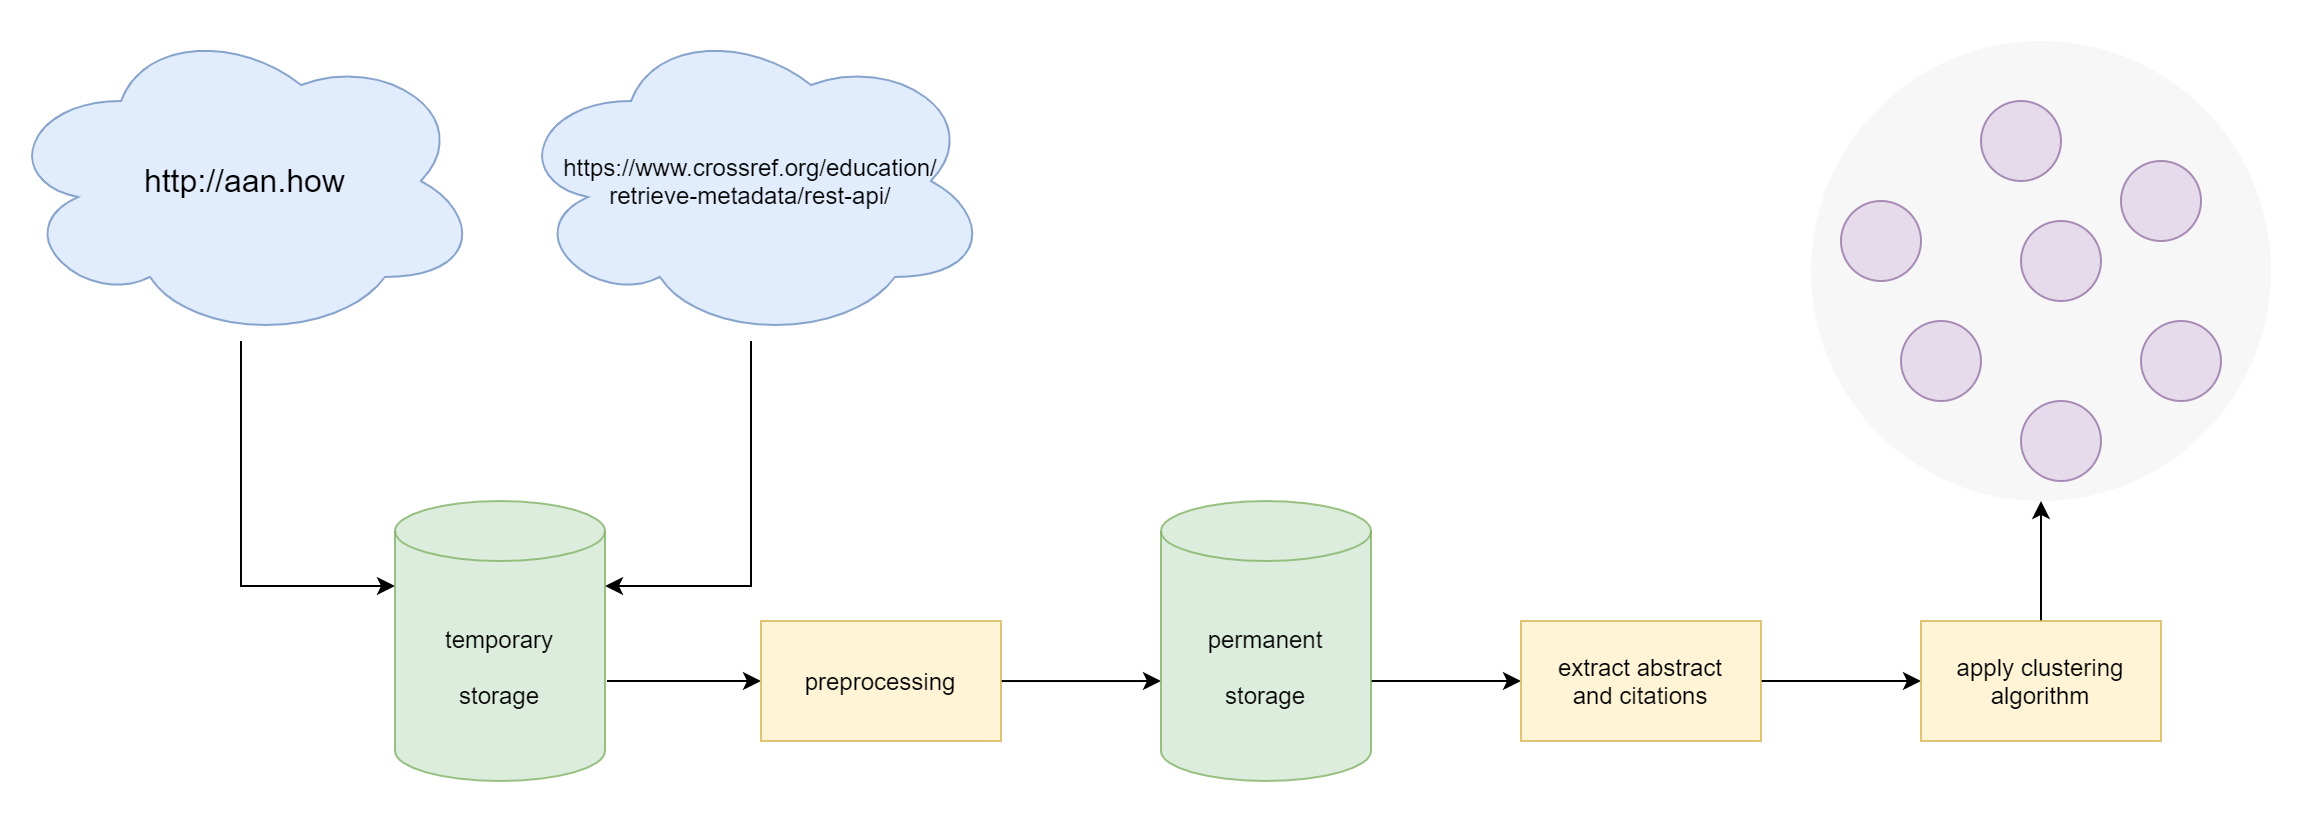
\includegraphics[width=\textwidth,keepaspectratio]{figures/pipeline}
    \caption[]{Coarse overview over the intended pipeline.}
    \label{fig:pipeline}
\end{figure}


\subsection{Data Set}
\label{subsec:data}
We have two main and one backup source of scientific papers:
\begin{itemize}
	\item Crossref \cite{crossref} is an official Digital Object Identifier Registration Agency that provides access to the full text of its registered research papers through their own API. Sending a HTTP request with "deep learning" as a query returns a JSON object with all the URLs to the PDFs of the registered papers found in Crossref's data base containing the terms "deep learning" in their title. The PDFs will then have to be converted into plain text.
	\item All About NLP \cite{aan} is a website maintained by Yale University's Learning and Information Group that provides a corpus consisting of over 400 scientific papers on NLP in plain text. Closer examination of the text files has, however, shown that most of them contain spelling mistakes.
	\item Journal of Machine Learning Research \cite{jmlr} is an international forum for the electronic and paper publication of scholarly articles in all areas of machine learning. The papers are available in pdf format, while the abstracts are in html format.
\end{itemize}


\section{Section}

Use sections to organize your contents. Read the project proposal guidelines available on Moodle to get more information on the contents your proposal should cover. Do not forget to cite online sources~\cite{WFR2017}, books~\cite{goldberg2017neural} or articles you are referencing! It may also be useful to integrate charts or figures in your proposal as seen in Figure~\ref{fig:example}.

\begin{figure}[h]
  \centering
  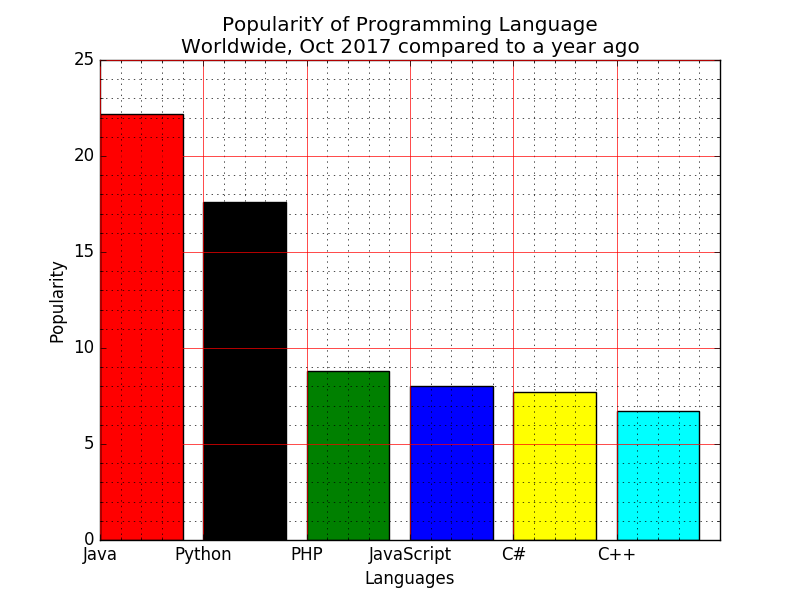
\includegraphics[scale=0.3]{figures/example_barchart}
  \caption[]{An example chart showing the change of popularity of various programming languages\footnotemark[1].}
  \label{fig:example}
\end{figure}

\footnotetext[1]{\url{https://www.w3resource.com/w3r_images/matplotlib-barchart-exercise-4.png}}

In the Latex source provided together with this PDF, you also find hints on how to work on one Latex project collaboratively.
=======
\section{Project Description}

\subsection{Main project goals}

practicalities of your approach, this time with a clearer focus on the application:
- make it easier for users to search and explore scientific papers belonging to a specific topic / theme
- create cluster representation that makes this easy to include in downstream tasks

Our main goal is to make it easier for users to search and explore scientific papers belonging to a specific topic or theme.
For this we want to specifically arrive at a clustering (representation) that, for one, separates the different documents into correct clusters, but is also easy to work with in downstream tasks (e.g. the mentioned inclusion in some search site).
To achieve this we basically interpret the steps mentioned in the subsection \ref{subsec:pipeline} as some coarse sub goals, which can then be worked on by different team members.
Some of these sub goals can also be further divided, for example downloading and preprocessing data from different sources or implementing distinct clustering algorithms can be done by a single team member respectively.

\subsection{Pipeline}
\label{subsec:pipeline}

Our pipeline will consist of the stages that can be seen in figure \ref{fig:pipeline}. First of all data from two different sources will be downloaded, temporarily stored and cleaned up to disregard records with missing data.
All cleaned up records will be stored permanently so we don't have to download and clean up the data every time we change some downstream settings. From this data storage the text we are going to use in the end will be extracted and some clustering algorithms will be used to build the final result.

\begin{figure}[ht]
    \centering
    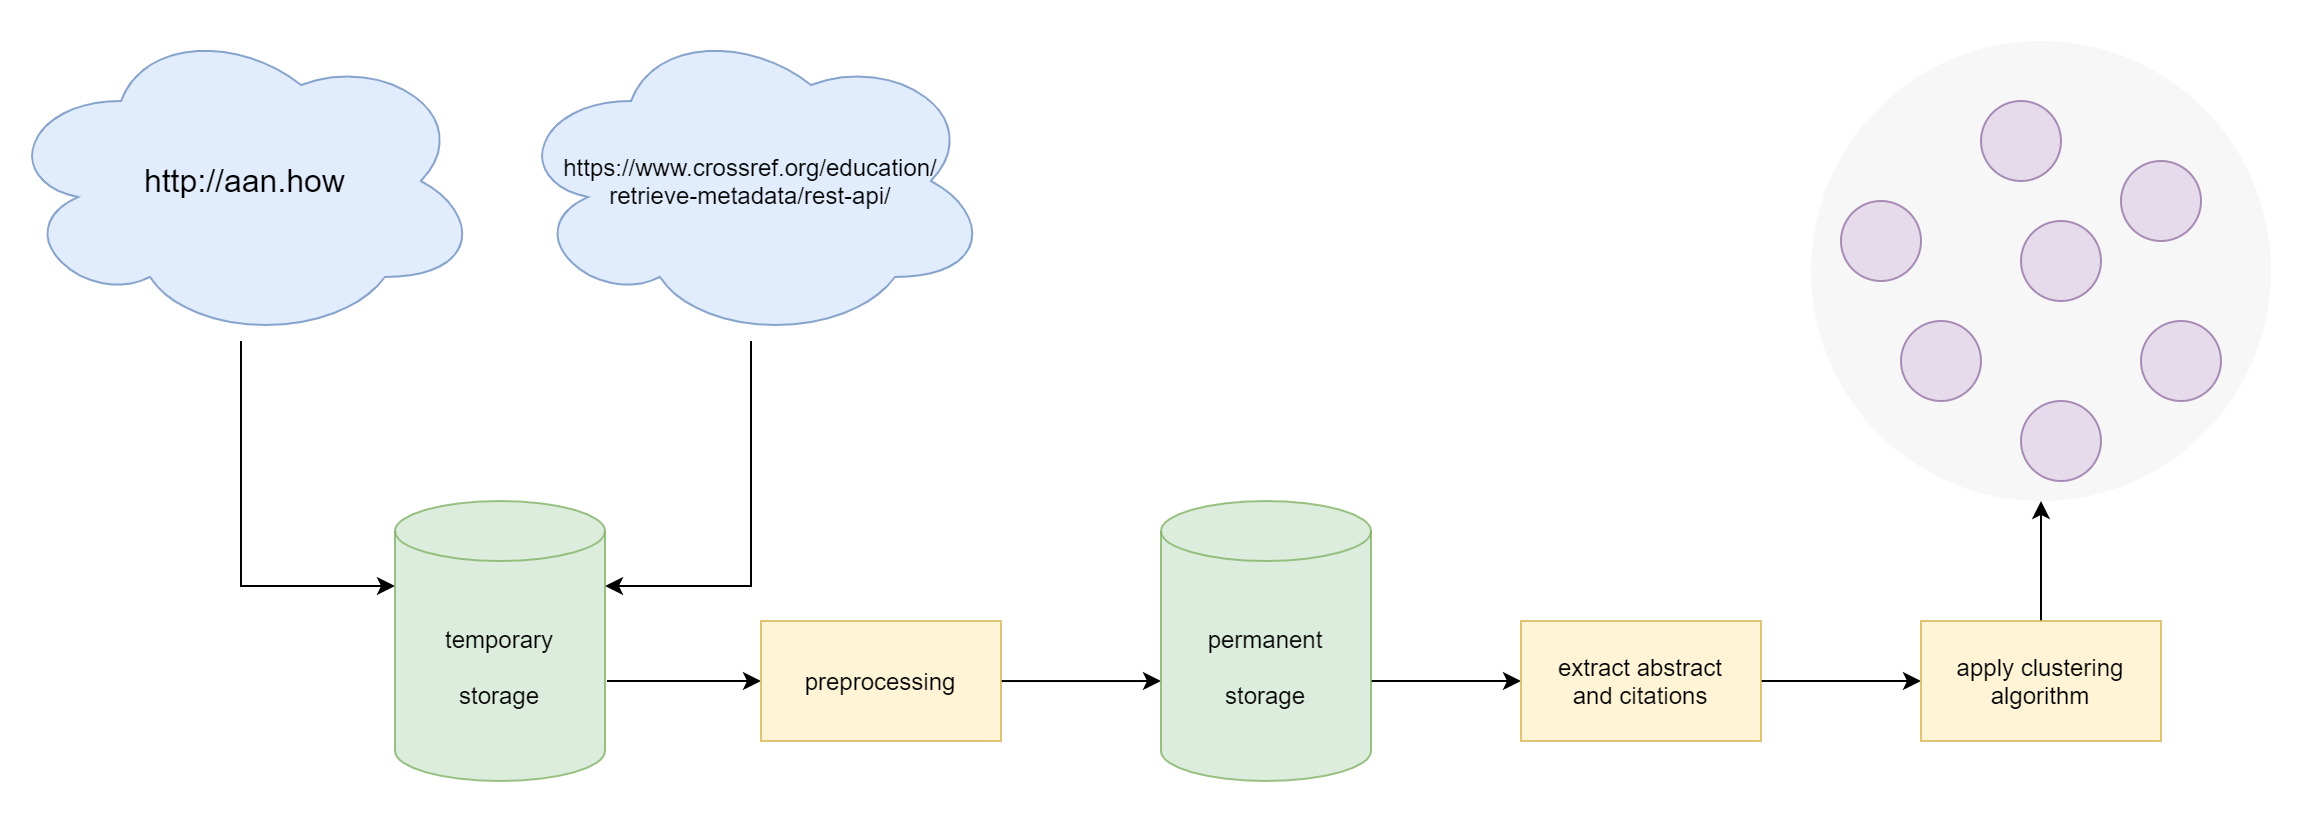
\includegraphics[width=\textwidth,keepaspectratio]{figures/pipeline}
    \caption[]{Coarse overview over the intended pipeline.}
    \label{fig:pipeline}
\end{figure}



%\subsection{Data Set}
\label{subsec:data}
We have two main and one backup source of scientific papers:
\begin{itemize}
	\item Crossref \cite{crossref} is an official Digital Object Identifier Registration Agency that provides access to the full text of its registered research papers through their own API. Sending a HTTP request with "deep learning" as a query returns a JSON object with all the URLs to the PDFs of the registered papers found in Crossref's data base containing the terms "deep learning" in their title. The PDFs will then have to be converted into plain text.
	\item All About NLP \cite{aan} is a website maintained by Yale University's Learning and Information Group that provides a corpus consisting of over 400 scientific papers on NLP in plain text. Closer examination of the text files has, however, shown that most of them contain spelling mistakes.
	\item Journal of Machine Learning Research \cite{jmlr} is an international forum for the electronic and paper publication of scholarly articles in all areas of machine learning. The papers are available in pdf format, while the abstracts are in html format.
\end{itemize}


\newpage %TODO Delete me!
\section{Evaluation}
\ref{sec:eval}
In this section, several evaluation approaches will be presented. Furthermore the whole processing pipeline is illustrated.

\subsection{Goal}
What is the goal of this work? Do we do unsupervised clustering of papers? Then we will have different evaluations on cluster statistics, number of clusters etc. 

Do we do supervised clustering/classification? Then we could compute something like a cross entropy loss, Kullback-Leibler divergence, etc.

I remember thatx our original idea was to utilize the existing key words to supervise our feature pipeline/ clustering algorithm. That means, that we define broader categories before and then compare relationships that we identify with the ones from the key words? We could also compute a similarity measure based on our ground truth and then compute a difference with the prediction.

\subsection{What evaluation losses are possible?}
When evaluating, we mean the direct comparison between our work and other works or the comparison of a ground truth and predictions. What metrics can be used for the task of key word generation? What losses are possible to compute for key word classification, general assignment problem?

Unsupervised: Label density, cluster variances, number of clusters, etc.

Supervised: Precision, Recall, F1-Score, KL-divergence, etc.

\subsection{Overall processing pipeline}
What is the overall processing pipeline? After identifying this, we can draw a nice picture. 

%NOTE Christian
% Do you use tikz for generatnig such charts or programs like inkspace. This is open for discussion and I would be glad for feedback how you do this in your own work. I personally, usually use inkscape and only tikz for very simple process flows. Alternatively I have all licenses you could possibly need (powerpoint , etc.).

\subsection{Outlook}
Outlook to evaluation on other tasks, that benefit from our task. This should be reorganized into the other .tex file in the end I guess. What I mean by this, is that we could evaluate our computed clusters on other tasks. Sort of how good recommended key words based on the classification are compared to ground truth key words. However, depending on how we organize our approach, this seems sort of like a full circle.

%NOTE Christian
% I will present some ideas on what else we can do with such a system to sell this to the TA's. Generating key words or clustering/assigning the text to some other sub category is the immediate goal/step. We can paint the bigger picture, where for a hot research topic, we can use this system to improve organizing research papers/trends into a better tree structure. Our system is a stepping stone into organizing the flood of papers in areas, such as Covid, Deep Learning, ..., you name it. After automatically assigning good key words to each paper/abstract, we can create a grouping/tree to link papers against each others. Direct contributions to our subtask are benefitting parent tasks, e.g. paper recommendation engines of journal hosts (arxiv, google scholar, etc.) and more. 

\newpage %TODO Delete me!

%\input{CH_outlook}
>>>>>>> 1a53390fd3f06031a005e6d4c8c3b4e23e6d98f2

%%%%%%%%%%%%%%%%%%%%%%%%%%%%%%%%%%%%%%%%%%%%%%%%%%%%%%%%%%%%

% The following is especially useful if you work together on one proposal or report, and want to alter its content independently from each other (e.g., to keep your commit history clean).

% Alternative: put content in separate files
% Check the difference between including these files using \input{filename} and \include{filename} and see which one you like better
%\chapter{Einleitung}\label{intro}
%\subsection{Introduction}

\subcomment{Written by Daniela Fichiu}
If you type a query like "how do I open the terminal on mac?" into Google, you already know what you want to find: a set of steps that will open a terminal on the screen.

Most would say doing homework is, on the best days, an unpleasant affair. But everyone would agree that writing an assignment for that one course you've always skipped is a chore. You most certainly do not understand the airy slides. Your only option is to search for materials on your own - extensive research is needed to find the materials that can fill all your knowledge gaps.

A student who wants to know more about text analytics might search for "text analytics" on Google Scholar. The query yields back 1.650.000 results, the top three being "Text Analytics with Python," "Text analytics in social media," and "Semantic interaction for visual text analytics." A subsequent query like "text analytics topics" yields back results with the following titles: "Analyzing educational comments for topics and sentiments: A text analytics approach" or "A text analytics approach for online retailing service improvement: Evidence from Twitter."

We know how time-consuming it is to spend hours on search engines or websites like Research Gate or Google Scholar looking for research papers, hoping for the best, but never quite finding the perfect materials.

Our project emerged from the need to find an easy way of exhaustively searching for scholarly literature while bringing to light the relations between the subfields of the research field of interest and other areas. Our goal is to provide a deeper understanding of the material to be searched for and easing up the process of finding information.

We propose a solution that clusters scientific texts into relevant subgroups. The subgroups can then be more easily presented to and explored by people looking for specific topics and terms.

We focus on a subset of around two thousand papers from the field of machine learning. We cluster the research papers, extract a ground truth using the papers' keywords, and compare the clustering results against the ground truth. We also prove that an unbalanced data set can have a significant impact on the clustering results. 

Even with the conclusions written down, we do not see our work as finished. The proposed pipeline could be usable on a broader range of fields. We also intend to balance our data set by adding research papers from other areas.

We also believe that our solution, supported by good group visualization tools and a user-friendly search interface, can be successfully integrated into a metasearch site.
%
%\chapter{Voraussetzungen}\label{bg}
%\input{background}

%%%%%%%%%%%%%%%%%%%%%%%%%%%%%%%%%%%%%%%%%%%%%%%%%%%%%%%%%%%%

% References (Literaturverzeichnis):
% see
% https://de.wikibooks.org/wiki/LaTeX-W%C3%B6rterbuch:_bibliographystyle
% for the different formats and styles

\bibliographystyle{plain}
% b) The File:
\bibliography{bibtex/references, bibtex/CH_ref}

\newpage

\begin{appendices}
    \section{Figures}
    \begin{figure}[ht]
        \centering
        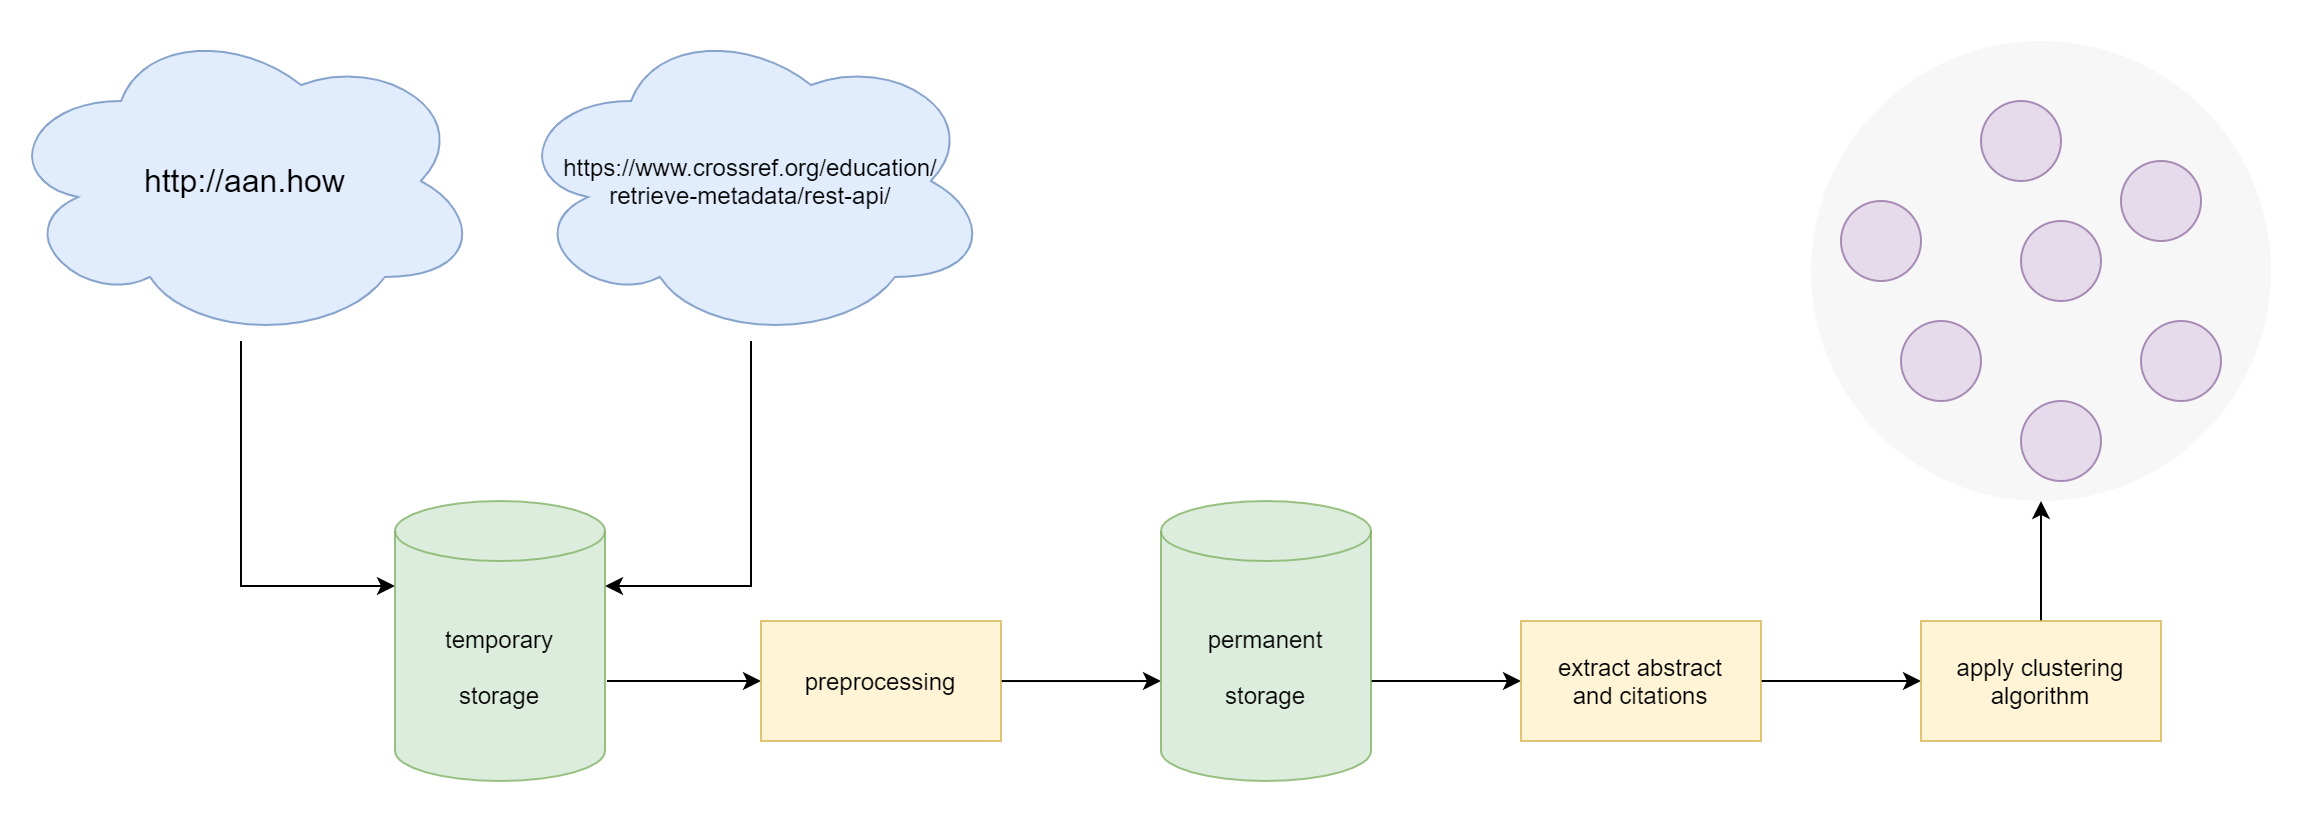
\includegraphics[width=\textwidth,keepaspectratio]{figures/pipeline}
        \caption[]{Coarse overview over the intended pipeline.}
        \label{fig:pipeline}
    \end{figure}
  \end{appendices}

\end{document}
